\documentclass[10pt, compress]{beamer}
\usetheme[conference=MST1-GPM17,venue=Culham, date=14/11/2017, titleprogressbar, logo=RFX-logo]{Eurof}
\usepackage{listings,amsmath,multimedia, amssymb}
\usepackage{../beamerclass/tangocolors}
\usepackage{../beamerclass/rfxcolor}
% for drawing
\usepackage{pgf}
\usepackage{tikz}
\usetikzlibrary{arrows,shapes,backgrounds}
\usepackage{../beamerclass/onimage}
\usepackage[export]{adjustbox}
\usepackage{bm}
% for font
\usepackage[absolute,overlay]{textpos}
  \setlength{\TPHorizModule}{1mm}
  \setlength{\TPVertModule}{1mm}

\usepackage[style=nature,citestyle=authoryear-comp,defernumbers=true,maxnames=2,firstinits=true,
uniquename=init,backend=bibtex8,arxiv=abs,mcite]{biblatex}
\bibliography{biblio}
\renewcommand*{\bibfont}{\footnotesize}
\renewcommand*{\citesetup}{\footnotesize}
\usepackage[export]{adjustbox}
\makeatother
\mode<presentation>
\makeatletter
% add a macro that saves its argument
\newcommand{\footlineextra}[1]{\gdef\insertfootlineextra{#1}}
\newbox\footlineextrabox
% for reducing font on a single slide
\newcommand\Fontvi{\fontsize{8}{7.2}\selectfont}
\title{{\small Filamentary transport in high-power H-mode conditions and in
  no/small-ELM regimes to predict heat and particle loads on PFCs for
  future devices}}
\date{{\footnotesize 14 November 2017}}
\author[N. Vianello and V. Naulin]{N. Vianello, V. Naulin for Topic-21
Scientific Team}
\begin{document}
\tikzstyle{every picture}+=[remember picture]
\maketitle
\begin{frame}{Scientific Team}
\begin{center}
  Jiri Adamek, Matteo Agostini, Diogo Aguiam, Scott Allan, Matthias Bernert, Daniel Carralero Ortiz, 
Stefan Costea, Istvan Cziegler, Hugo De Oliveira, Joaquin Galdon-Quiroga, Gustavo Grenfell, Antti Hakola, 
Codrina Ionita-Schrittwieser, Heinz Isliker, Alexander Karpushov, Jernej Kovacic, Benoît Labit, Florian Laggner, Jens Madsen, 
Roberto Maurizio, Ken McClements, Fulvio Militello, Jeppe Miki Busk Olsen, Jens Juul Rasmussen, Timo Ravensbergen, Bernd Sebastian Schneider, Roman Schrittwieser, Jakub Seidl, Monica Spolaore, Christian Theiler, Cedric Kar-Wai Tsui, Kevin Verhaegh, Jose Vicente, 
Nickolas Walkden, Zhang Wei, Elisabeth Wolfrum
\end{center}
\end{frame}

\begin{frame}{2017 Top Objectives 
    12.12.2016}
  \Fontvi
\vspace{-1cm}
Deliverables listed during the call for manning of last December 
\begin{enumerate}
\item \only<2>{\color{ta3chameleon}} Cross-machine L-Mode
  shoulder dependence on current both at constant B$_t$ and at
  constant $q_{95}$. Rationale: disentangle the effect of current and
  parallel connection length
\item \only<2>{\color{taorange}}Establish robust scenario for density
  shoulder profile in H-Mode and establish dependence on
  fuelling/neutral profiles/divertor condition
\item \only<2>{\color{ta3chameleon}}Use the new HHF probe on AUG to study
  filamentary transport under high-power H-Mode conditions \only<2>{\color{consorziored}}and under
  different plasma configurations (SN, DN)
\item \only<2>{\color{taorange}}Study the role of ELM regimes,  neutral
  compression and particle density in filamentary transport and
  related shoulder formation
\item \only<2>{\color{taorange}} Identify the contribution of
  collisionality and seeding on filamentary transport and related
  shoulder formation
\item \only<2>{\color{consorziored}}Determine the effect of filaments and
  shoulder formation on target heat loads in different H-mode plasmas
\end{enumerate}
\onslide<2>{
  So far H-Mode operation has been limited to AUG since no operational
  scenario in high-density NBH heated plasma on TCV has been established
}
\end{frame}

\begin{frame}{L-Mode analysis: I$_p$ scan at constant q$_{95}$}
\Fontvi
  \vspace{-1cm}
  \begin{columns}    
  \begin{column}{0.65\textwidth}
    \centering{\includegraphics<1>[height=.8\textheight]{../../Experiments/AUG/analysis/pdfbox/EquilibraLparallelConstantQ95}}
    \includegraphics<2>[height=.81\textheight]{../../Experiments/AUG/analysis/pdfbox/GeneralIpScanConstantq95}
    \centering{\includegraphics<3>[height=.85\textheight]{../../Experiments/TCV/analysis/pdfbox/EquilibriaLparallelConstantQ95}}
    \centering{\includegraphics<4>[height=.9\textheight]{../../Experiments/TCV/analysis/pdfbox/CurrentScanConstantQ95}}
    \centering{\includegraphics<5>[width=\textwidth]{../../Experiments/AUG/analysis/pdfbox/IpConstantQ95_Profiles_UsDiv}}
    \centering{\includegraphics<6>[width=\textwidth]{../../Experiments/AUG/analysis/pdfbox/n0_CurrentScanConstantQ95}}
    \centering{\includegraphics<7>[width=.6\textheight]{../../Experiments/AUG/analysis/pdfbox/RadiationPeakDensityIpScan_constantQ95Zoom}}
    \centering{\includegraphics<8>[width=\textwidth]{../../Experiments/TCV/analysis/pdfbox/IpConstantq95_samedensity}}
    \centering{\includegraphics<9>[width=\textwidth]{../../Experiments/TCV/analysis/pdfbox/CompareTargetProfilesConstantQ95}}
    \centering{\includegraphics<10>[width=\textwidth]{../../Experiments/AUG/analysis/pdfbox/BlobSizeCurrentScanConstantQ95}}
    \centering{\includegraphics<11>[width=\textwidth]{../../Experiments/AUG/analysis/pdfbox/GPI_blobs_AUG}}
    \centering{\includegraphics<12>[width=\textwidth]{../../Experiments/TCV/analysis/pdfbox/LambdaSizeIpScanConstantQ95}}
    
  \end{column}
  \begin{column}{0.35\textwidth}
    \begin{itemize}
      \item<1|only@1> AUG: All the shots were performed in the so-called
        Edge Optmized Configuration (EOC) shape. 
      \item<1|only@1> AUG: We matched correctly the shape and the L$_{\parallel}$
        here shown from outer divertor plate up to X-point 
      \item<2|only@2> AUG: The scan was performed with similar puffing
        rates for intermediate and higher current (0.8-1
        MA) whereas we reduced it at lower current to avoid early
        disruption
      \item<2|only@2> AUG: The total power (Ohmic plus NBI) was kept
        constant throughout the scan
      \item<2|only@2> AUG: We have comparable edge density, divertor neutral
        pressure and divertor temperature
      \item<3|only@3> TCV: We repeat the same excercise at TCV with a
        slight difference in the profile of parallel connection
        length. This required operation at unusual low toroidal field
        (up to 0.8T)
      \item<4|only@4> TCV: no additional heating
        has been used. Nevertheless the difference in power crossing the separatrix
        is small
      \item<4|only@4> TCV: The difference in target pressure similar
        to AUG behavior. 
      \item<5|only@5> AUG: At comparable edge density Upstream profiles are
        different with the tendency to develop shoulder easier at
        lower current. \alert{We have flattening of the upstream
          profiles only when $\Lambda_{div}$ is well above one on all
          the profile}
      \item<6|only@6> AUG: Neutrals estimated using calibrated D$_{\alpha}$
        cameras coupled with values of density and temperature at the
        target suggest a larger neutral density at lower current (even
        with comparable values of edge electron density)
      \item<7|only@7> AUG: At all the current a clear roll-over in
        peak density at the target observed and we can also track the radiation
        front move away from target earlier in density at lower current
      \item<8|only@8> TCV: This tendency is not observed for TCV where
        profiles seem resilient to modification of Bt even though we
        reached pretty high value of $\Lambda_{div}$ all along the profile.
      \item<9|only@9> TCV: This is due to the fact that we can't
        observed during the density ramp any signature of rollover or detachment,
        \alert{whereas upstream profile modification at TCV are only observed
        well after rollover}
      \item<10|only@10> AUG: There is the tendency towards larger blobs
        at lower current at all values of $\Lambda_{div}$
      \item<11|only@11> AUG: This need to be further confirmed
        independently by GPI measurements (I. Cziegler \textit{et al.}). The present setup allows
        for space resolution of the order of mm with a 397 kframe/s
        sampling rate. Small amount of He gas flux needed ($\sim
        1.5e^{17} atoms/ms$)
      \item<12|only@12> TCV: this is not confirmed for TCV where blob
        sizes is rather constant over a rather large range of
        $\Lambda_{div}$. At the same time we do not observe target
        density rollover neither upstream profile flattening 
      \end{itemize}
    \end{column}
\end{columns}
\end{frame}

\begin{frame}{L-Mode analysis: I$_p$ scan at constant B$_{t}$}
\Fontvi
  \vspace{-1cm}
  \begin{columns}    
  \begin{column}{0.65\textwidth}
    \centering{\includegraphics<1>[height=.8\textheight]{../../Experiments/AUG/analysis/pdfbox/EquilibraLparallelConstantBt}}
    \centering{\includegraphics<2>[height=.8\textheight]{../../Experiments/AUG/analysis/pdfbox/GeneralIpScanConstantBt}}
    \centering{\includegraphics<3>[height=.85\textheight]{../../Experiments/TCV/analysis/pdfbox/EquilibriaLparallelConstantBt}}
    \centering{\includegraphics<4>[height=.9\textheight]{../../Experiments/TCV/analysis/pdfbox/CurrentScanConstantBt}}
    \centering{\includegraphics<5>[width=\textwidth]{../../Experiments/AUG/analysis/pdfbox/IpConstantBt_Profiles_UsDiv}}
    \centering{\includegraphics<6>[width=\textwidth]{../../Experiments/AUG/analysis/pdfbox/n0_CurrentScanConstantBt}}
    \centering{\includegraphics<7>[width=.65\textheight]{../../Experiments/AUG/analysis/pdfbox/RadiationPeakDensityIpScan_constantBTZoom}}
    \centering{\includegraphics<8>[width=\textwidth]{../../Experiments/TCV/analysis/pdfbox/IpConstantBt_samedensity}}
    \centering{\includegraphics<9>[width=\textwidth]{../../Experiments/TCV/analysis/pdfbox/CompareTargetProfilesConstantBt}}
    \centering{\includegraphics<10>[width=\textwidth]{../../Experiments/AUG/analysis/pdfbox/BlobSizeCurrentScanConstantBT}}
    \centering{\includegraphics<11>[width=\textwidth]{../../Experiments/TCV/analysis/pdfbox/LambdaSizeIpScanConstantBt}}
    
  \end{column}
  \begin{column}{0.35\textwidth}
    \begin{itemize}
      \item<1|only@1> AUG: We matched correctly the shape the parallel
        connection length L$_{\parallel}$ is modified consistently
      \item<1|only@1> AUG: The scan was performed with similar puffing rate (0.8-1
        MA) whereas we reduced it at lower current to avoid early disruption
      \item<2|only@2> AUG: We have comparable edge density and divertor neutral
        pressure even though pressure increase earlier at higher current
      \item<2|only@2> AUG: The total power (Ohmic plus NBI) was kept
        constant throughout the scan
      \item<3|only@3> TCV: We repeat the same excercise at TCV with a
        consistent variation of parallel connection
        length. \alert{L$_{\parallel} at TCV is almost one order of
          magnitude larger than AUG$}
      \item<4|only@4> TCV: no additional heating
        used. Nevertheless the difference in power crossing the separatrix
        is small
      \item<4|only@4> TCV: Neutral compression is roughly constant between
      \item<5|only@5> AUG: At comparable edge density Upstream profiles are
        different with the tendency to develop shoulder easier at
        lower current. \alert{We have flattening of the upstream
          profiles only when $\Lambda_{div}$ is well above one on all
          the profile}
        \item<6|only@6> AUG: Neutrals at lower current are substantially
          higher even with similar edge density profiles.
        \item<7|only@7> AUG: Similarly to the observation at constant
          q$_{95}$ target peak density rollover and radiation movement
          from the target occurs earlier in density at lower plasma current
      \item<8|only@8> TCV: This tendency is substantially confirmed at
        TCV even though larger scatter in the data has been
        obtained. To be combined with similar experiment performed
        under MST1-2015  
      \item<9|only@9> TCV: This is consistent with onset of detachment
        (at least in intermediate and lower current)
      \item<10|only@10> AUG: While the general observation of increasing
        blob size with $\Lambda_{div}$ is confirmed there are no
        differences between the current
      \item<11|only@11> TCV: Even at TCV no big differences in blob
        size has been observed. Statistics should be increased
        including past experiment from MST1-2015 
      \end{itemize}
    \end{column}
\end{columns}
\end{frame}

\begin{frame}{LSN \textit{vs} Double null on TCV}
%  \begin{columns}
%    \begin{column}{0.5\textwidth}
      \centering{\includegraphics<1>[width=.6\textwidth]{../../Experiments/TCV/analysis/pdfbox/CompareTargetProfilesLSN-DN}}
      \centering{\includegraphics<2>[width=.8\textwidth]{../../Experiments/TCV/analysis/pdfbox/DNRadiation_58623}}
      \centering{\includegraphics<3>[width=.8\textwidth]{../../Experiments/TCV/analysis/pdfbox/DNRadiation_58624}}
      \centering{\includegraphics<4>[width=.8\textwidth]{../../Experiments/TCV/analysis/pdfbox/LambdaSizeLSN-DN}}
%    \end{column}
%    \begin{column}{0.5\textwidth}
      \begin{itemize}
        \item<1|only@1> Comparing similar L-Mode density ramp at same
          current in LSN and DN with ion $\mathbf{B}\times\nabla B$
          pointing towards the floor. Lower ion flux to lower target
          observed in DN and profiles before rollover seem more broad
          in LSN. After rollover the profiles are actually similar
      \item<2|only@2>  From bolometry we can observe an
          unbalanced movement of the radiation front suggesting a non
          perfectly balanced DN
      \item<3|only@3> This is confirmed at higher current where the
        more active X-point is the upper one with a consequent higher
        radiation from bolometry chords
      \item<4|only@4> No clear difference in blob size but needs
        further investigation  
      \end{itemize}
%    \end{column}
%  \end{columns}
\end{frame} 

\begin{frame}{H-Mode investigation: puffing location}
\Fontvi
  \vspace{-1cm}
\begin{columns}
  \begin{column}{0.65\textwidth}
    \centering{\includegraphics<1>[height=0.85\textheight]{../../Experiments/AUG/analysis/pdfbox/PuffingLocation}}
    \centering{\includegraphics<2>[width=\textwidth]{../../Experiments/AUG/analysis/pdfbox/CompareShot34276_34277}}
    \only<3>{
      \begin{tikzonimage}[width=\textwidth]{../../Experiments/AUG/analysis/pdfbox/EvolutionEdgeProfiles_34276_34277}
        \draw [->, ultra thick, white] (0.2, 0.45) -- (0.3, 0.55);
        \draw [->, ultra thick, white] (0.62, 0.45) -- (0.72, 0.55);
      \end{tikzonimage}   
    }
  \end{column}
  \begin{column}{0.35\textwidth}
    \begin{itemize}
      \item<1-> Similar puff from Lower and Upper divertor valves
        (\alert{we asked for divertor/midplane valves})
      \item<2-> Discharge with a total amount 6.5 heating power
        with equivalent behavior also in the lower divertor
        independently from the puffing location
      \item<3-> Edge density profiles from Li-Beam evolution are
        pretty similar
      \item<3|alert@3> Similar behavior observed from RIC Antenna 4
        for the available shot
    \end{itemize}
  \end{column}
\end{columns}
\end{frame}

\begin{frame}{Compare fueling with/without cryopumps}
\Fontvi
  \vspace{-1cm}
\begin{columns}
  \begin{column}{0.65\textwidth}
    \centering{\includegraphics<1>[width=\textwidth]{../../Experiments/AUG/analysis/pdfbox/CompareShot34276_34278}}
    \centering{\includegraphics<2>[height=.65\textheight]{../../Experiments/AUG/analysis/pdfbox/PuffingIpolsola34276_34278}}
    \only<3>{
    \begin{tikzonimage}[width=\textwidth]{../../Experiments/AUG/analysis/pdfbox/EvolutionEdgeProfiles_34276_34278}
      \draw [->, ultra thick, white] (0.2, 0.45) -- (0.3, 0.55);
      \draw [->, ultra thick, dashed, red] (0.62, 0.45) -- (0.72, 0.55);
    \end{tikzonimage}}
  \centering{\includegraphics<4>[height=.85\textheight]{../../Experiments/AUG/analysis/pdfbox/Shot_34276_34278_InterELMprofiles}}
  \end{column}
  \begin{column}{0.35\textwidth}
    \begin{itemize}
    \item<1-> Same fueling but with cryo-pumps
      \item<1-> H-5 density is different and remain constant, both
        divertor and midplane pressure are reduced (to 1/3
        approximately) no sign of detachment
      \item<2-> Different ELMy regimes reached with reduced size and
        increased frequency without the cryopumps
      \item<3-> Also with this amount of fueling weaker indication of SOL
        saturation observed as confirmed by Li-Beam and by RIC (Antenna 4)
      \item<4> Inter-ELM resolved profile suggest a flattening even
        with the cryompumps still even though $\Lambda_{div}$ is
        marginal above 1 only in the near SOL
        
    \end{itemize}
  \end{column}
\end{columns}
\end{frame}

\begin{frame}{Matching scenarios with cryo-pumps}
\Fontvi
  \vspace{-1cm}
\begin{columns}
  \begin{column}{0.65\textwidth}
    \centering{\includegraphics<1>[width=\textwidth]{../../Experiments/AUG/analysis/pdfbox/CompareShot34276_34281}}
    \centering{\includegraphics<2>[width=\textwidth]{../../Experiments/AUG/analysis/pdfbox/PuffingIpolsola34276_34281}}
    \centering{\includegraphics<3>[width=\textwidth]{../../Experiments/AUG/analysis/pdfbox/EvolutionEdgeProfiles_34276_34281}}
    \centering{\includegraphics<4>[height=0.9\textheight]{../../Experiments/AUG/analysis/pdfbox/Shot_34278_34281_InterELMprofiles}}
    \centering{\includegraphics<5>[height=0.9\textheight]{../../Experiments/AUG/analysis/pdfbox/CompareCas34278_34281}}
  \end{column}
  \begin{column}{0.35\textwidth}
    \begin{itemize}
      \item<1-> To match similar edge density and divertor pressure
        and to reach the same level of detachment we increase the
        fueling by almost a factor of 3, increasing also the rate. In
        addition to that we also increase substantially the N
        puffing. \alert{Degraded H-Mode reached earlier in density
          without the cryopumps}
      \item<2-> Similar ELMy behavior obtained during the density ramp  
      \item<3-> Now the scenario suggest a strong profile flattening
        even with the cryopumps
       \item<4-> Inter-ELM resolved Li-Be profiles confirm this with
         shoulder formed with similar strength even with the cryopumps
         in operation.
         \item<5> We can also confirm that additional fueling change
           substantially the blob size which increases consistently
           with the modification of $\Lambda_{div}$
    \end{itemize}
  \end{column}
\end{columns}
\end{frame}

\begin{frame}{Fast electron generation (K. McClements \textit{et al})}
\Fontvi
  \begin{columns}
    \begin{column}{0.5\textwidth}
      \centering{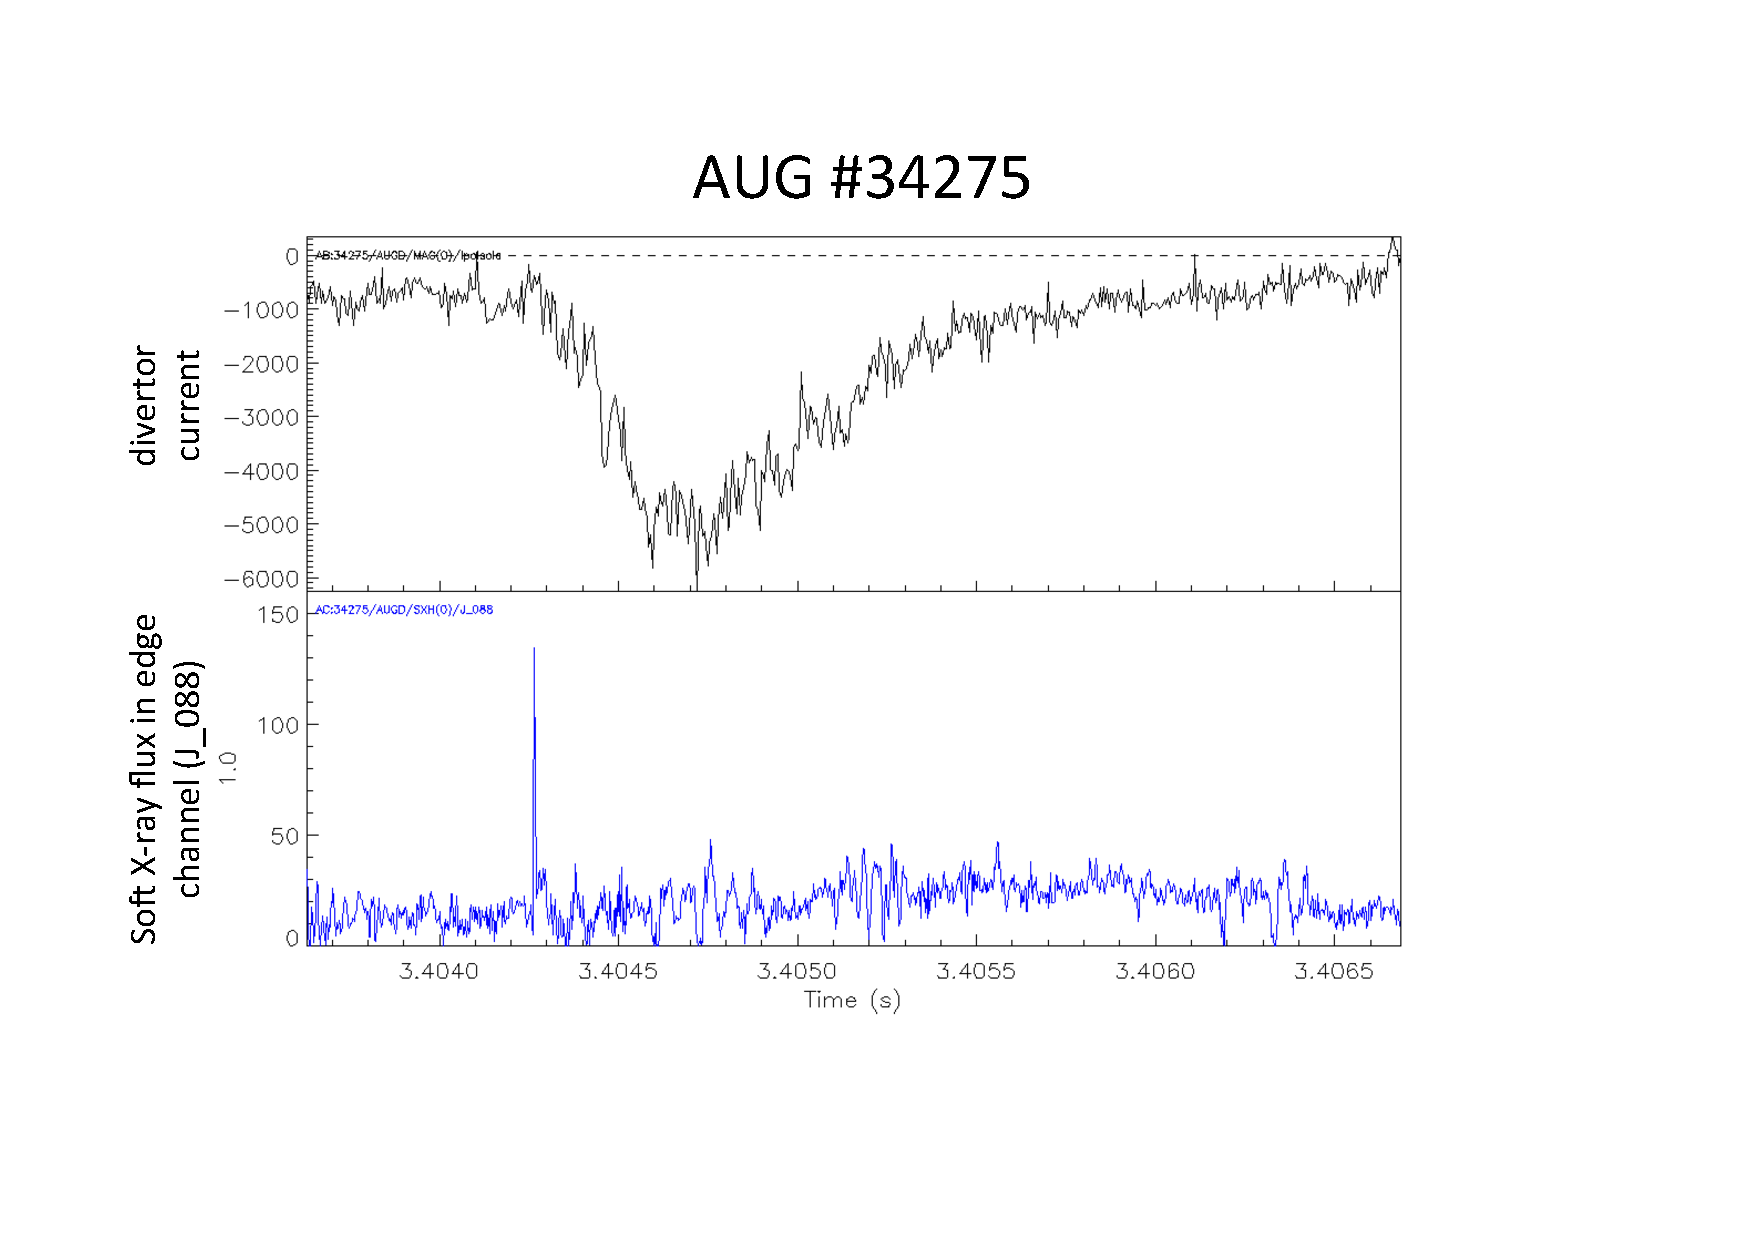
\includegraphics[width=\textwidth]{../../Experiments/AUG/analysis/pdfbox/SXR_ken}}
    \end{column}
    \begin{column}{0.5\textwidth}
\begin{itemize}
      \item Bursts of nonthermal 2nd harmonic electron cyclotron emission and edge soft X-ray emission often occur at start of ELM filament eruption in low collisionality AUG pulses – evidence of filament reconnection
\item Soft X-ray bursts were seen at start of ELM filament eruption in T21-AUG pulses, but not ECE bursts, probably due to higher collisionality in these pulses
\item Peak nonthermal ECE emission appears to originate from top of pedestal
\item Work is ongoing to determine conditions for occurrence of ECE \& SXR bursts, e.g. in terms of pedestal collisionality – there is no clear correlation between ELM size \& SXR flux
\end{itemize}
\end{column}

  \end{columns}
\end{frame}

\begin{frame}{Cross-machine: different divertor geometry}
  \begin{columns}
    \begin{column}{0.5\textwidth}
  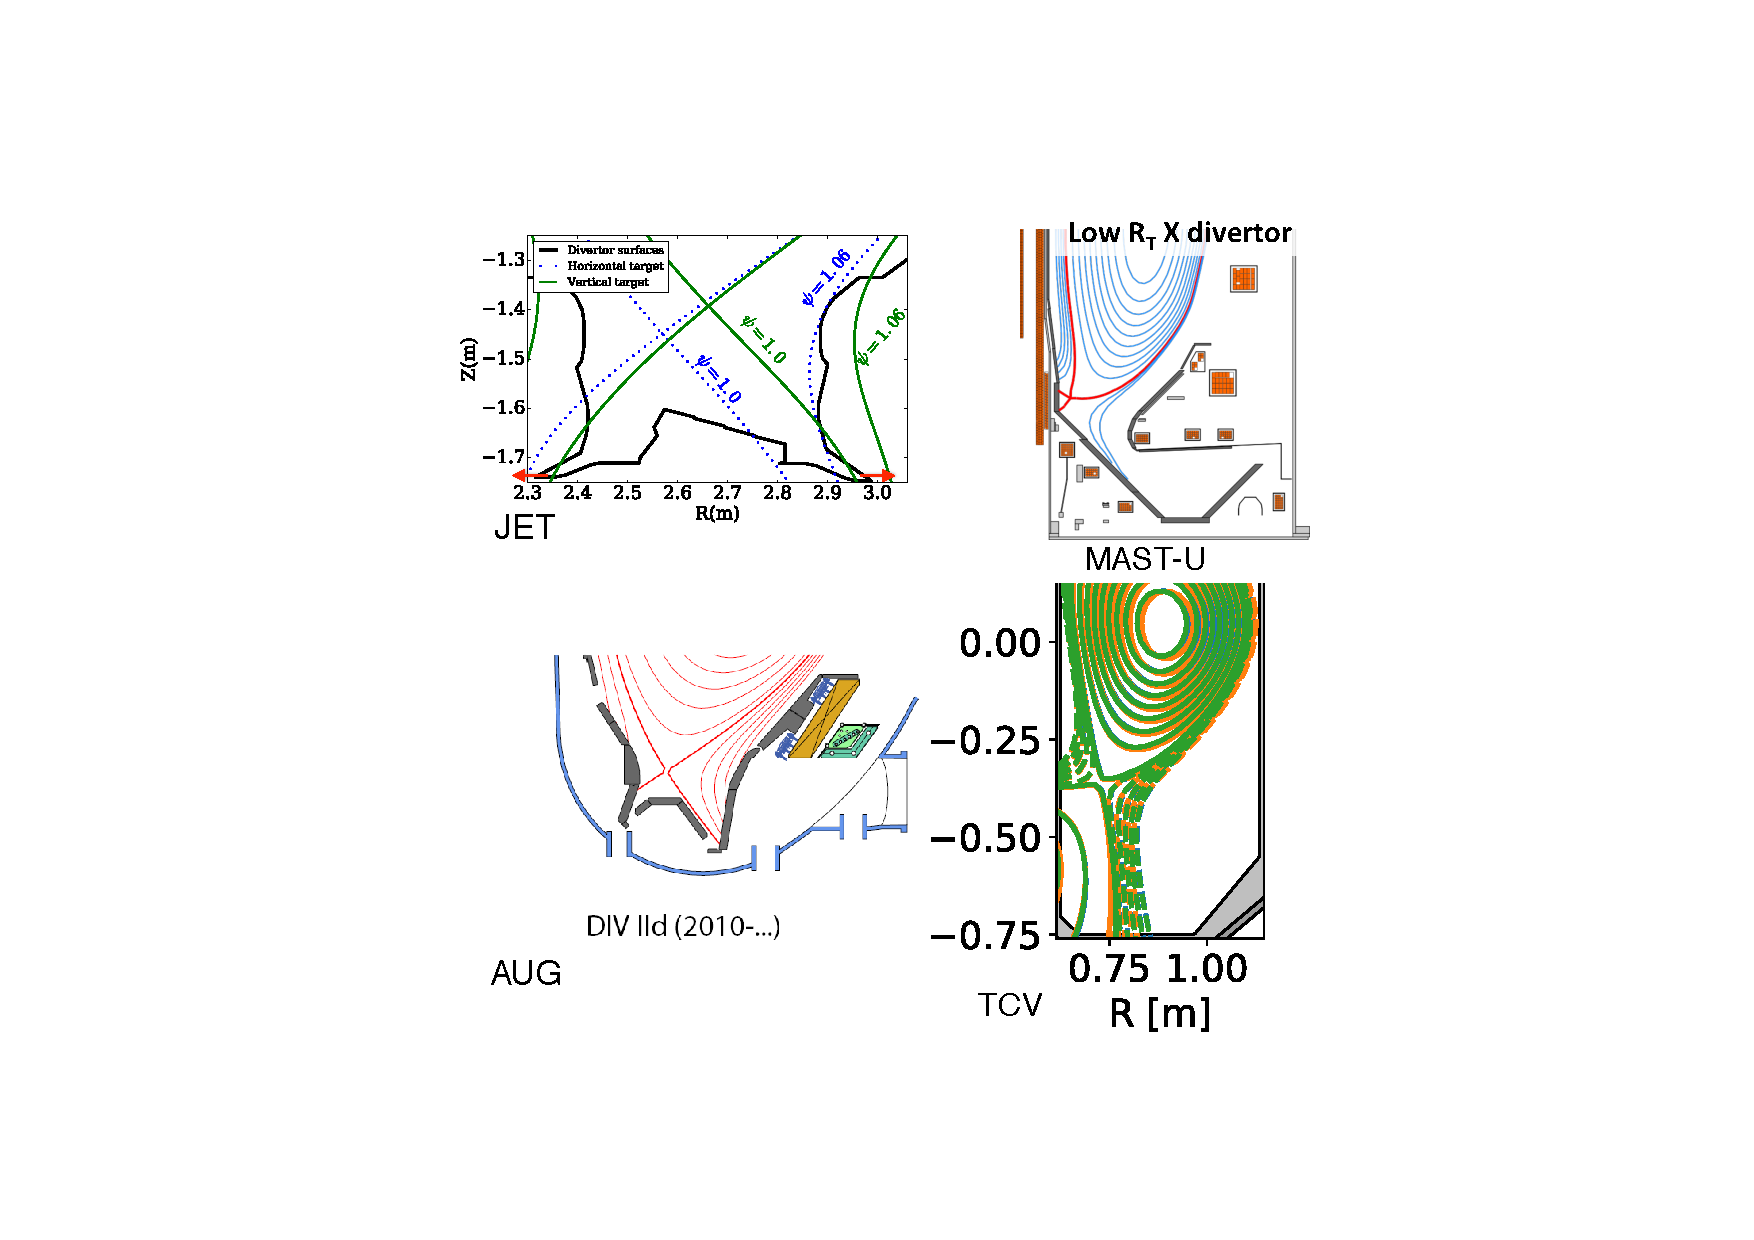
\includegraphics[width=\textwidth]{../generalFigures/Divertors}
\end{column}
\begin{column}{0.5\textwidth}
  \begin{itemize}
    \item Cross-machine experiments (including comparison with
      possible JET experiment) could help to disentangle how divertor
      geometry influence upstream profiles in term of neutral
      compression and recycling
    \item \alert{f.x. Vertical target on JET and AUG has very
        different behavior in terms of shoulder formation}
    \end{itemize}
  \end{column}
\end{columns}
\end{frame}

\begin{frame}{Program for 2018: AUG}
  \begin{itemize}
     \item X-point manipulator (NPH ?) simultaneously with MEM
     \item X-point vertical shift in order to have SP at different
	vertical height at the target. \alert{We will observe similar
          observation as obtained in JET when moving from horizontal
          to vertical target?}
     \item DN discharges. With slow movement of the second X-point into the vessel
	to be performed at constant power/density where shoulder
        alreay exists. \alert{This is mandatory to complement the
          information obtained on TCV}
     \item USN with midplane/X-point manipulator to monitor the
       upstream SOL 
     \item Heat load
\end{itemize}
 \end{frame}
 \begin{frame}{MST2-NPH}
   \begin{columns}
     \begin{column}{0.5\textwidth}
       \centering{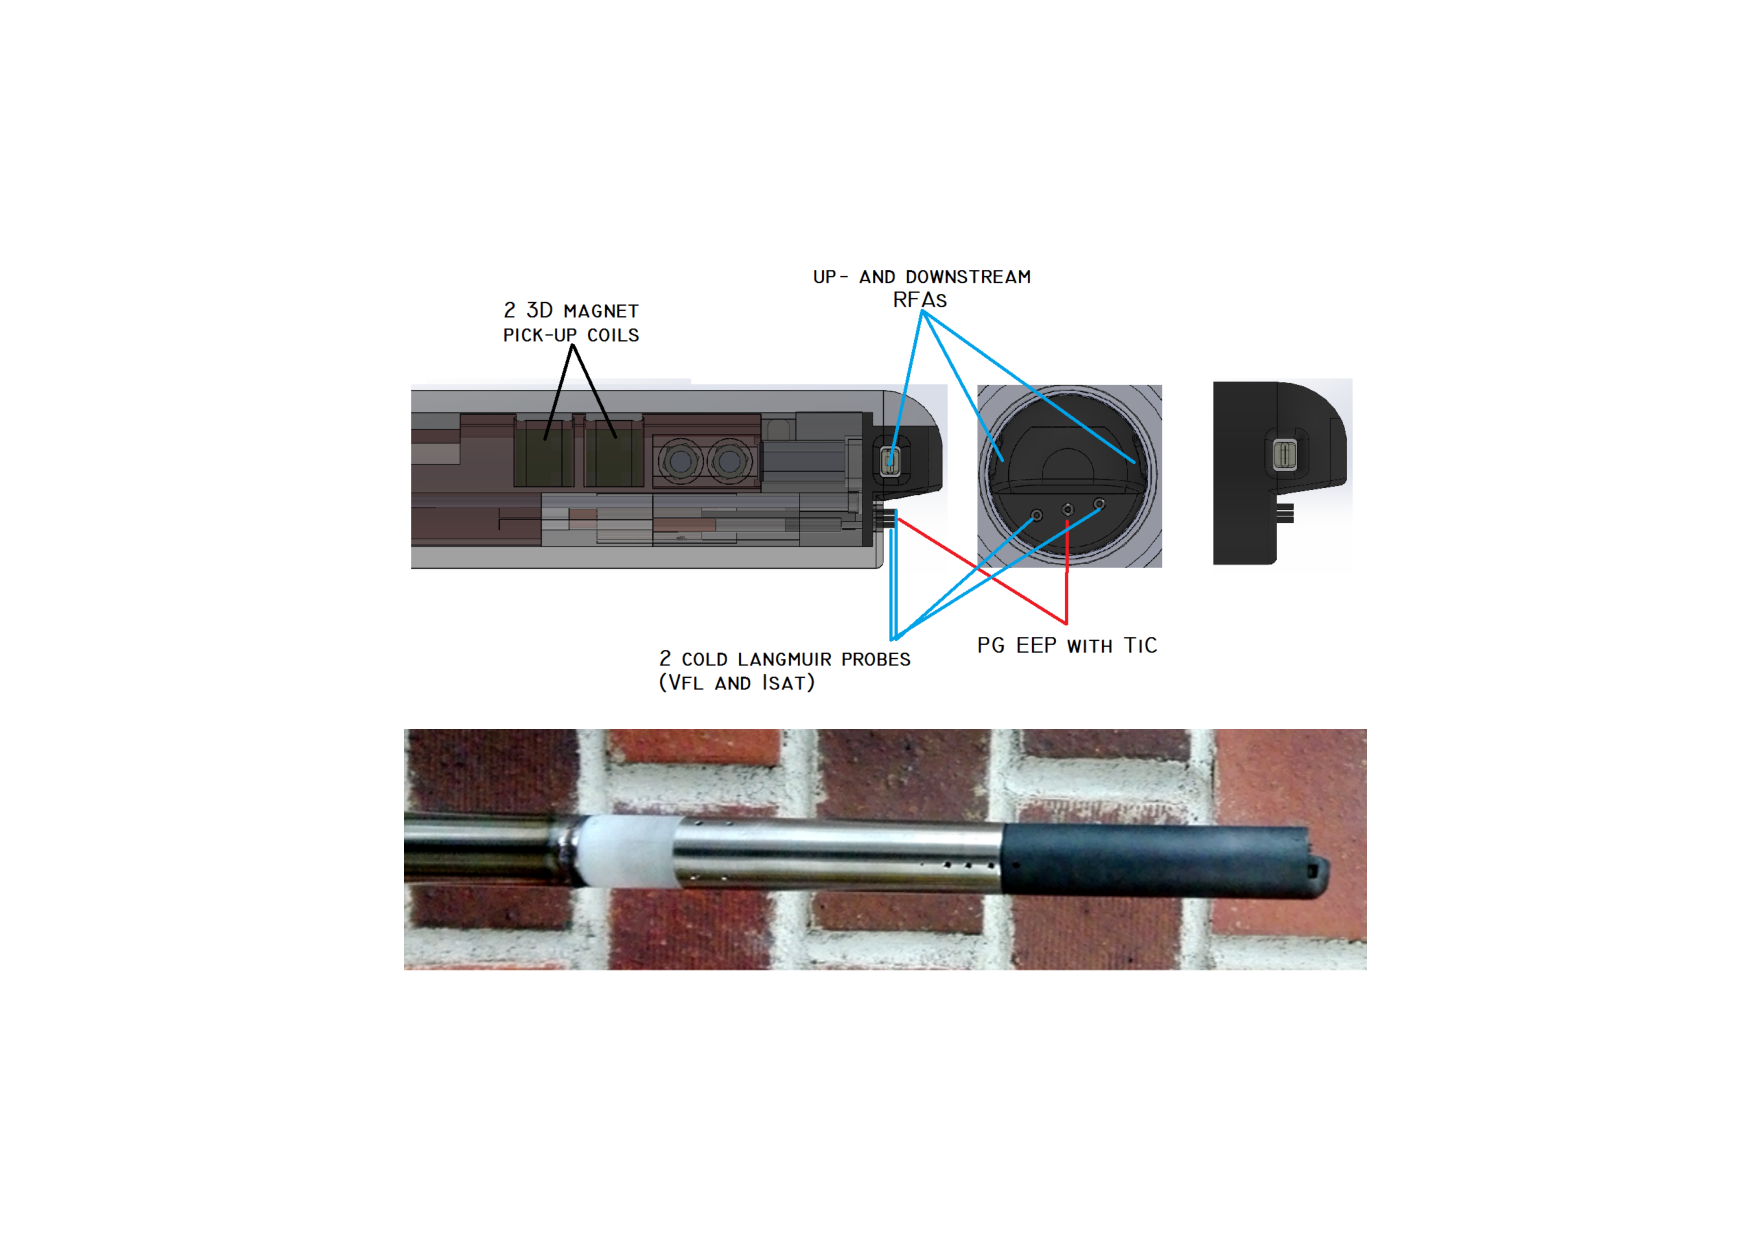
\includegraphics[width=\textwidth]{../../Experiments/AUG/analysis/pdfbox/NPH_2018}}
     \end{column}
     \begin{column}{0.5\textwidth}
       \begin{itemize}
         \item MST2 founded project for the realization of a New Probe
           Head (NPH) (C. Ionita,  B. Schneider \textit{et al})
         \item Simultaneous information on Ion temperature (2 RFAs),
           Plasma potential and electron temperature (Emissive probe
           coupled with floating potential) and magnetic fluctuations
           from 2 3-axial magnetic pick up coil
         \item Potentially tested on TCV beginning of 2018 and then
           moved to other MST1 devices
       \end{itemize}
     \end{column}
   \end{columns}
 \end{frame}
 
\begin{frame}{Program for 2018: TCV}
  \begin{itemize}
     \item \textcolor{consorziored}{H-Mode} 
      \item Long divertor legs (probe in the lower port) to check if
        increase of filamentary transport along the divertor leg
        exists in high density scenarios
      \item \textcolor{taorange}{SnowFlake to monitor the fluctuations in between the 2 separatrix
	to be done in high density discharges}
       \item \textcolor{taorange}{Try to move the second X-point in SN divertor at a different
	Z position while keeping the same radial distances between the
	points}
\end{itemize}
\end{frame}

\begin{frame}{Program for 2018: MAST-U}
  \begin{itemize}
      \item Current scan at constant q95/constant Bt
      \item Influence of neutral recycling source in establishing upstream profiles
	and comparison between Low-RT and Vertical target. Look also a
        the heat loads
      \end{itemize}
\end{frame}

\begin{frame}{Code requirements}
  \begin{itemize}
    \item Dedicated simulations with first principles codes (GBS,
      HESEL)
    \item Check if trends can be reproduced
    \item potential input for future experiments regarding role of
        f.x. neutrals and recycling
  \end{itemize}
\end{frame}
\end{document}

